\section{Must know}

\subsection{Line equation}

If the normal vector is (a,b) and given a point (c,d), the line equation is
\(a(x-c) + b(y-d)=0\)


\subsection{Matrix properties}

\subsubsection{Homography matrix}
H has 8 degrees of freedom because it's defined up to scale.
2 for scale, 2 for rotation, 2 for translation, 2 for ``line at infinity'' to
finite. Has rank 3.

\subsubsection{Isometry matrix}
Has 3 DoF, 1 rotation, 2 translation

\subsubsection{Similarity matrix}
4 DoF, 1 scale, 1 rotation, 2 translation

\subsubsection{Affine matrix}
6 DoF, 2 scale, 2 rotation, 2 translation

\subsubsection{Fundamental matrix}
Has 7 DoF. 1 DoF is subtracted because it's defined up to scale, 1 because it's
a rank 2 matrix. Because F is singular, it can't be of rank 3. Because it
represents a mapping from a 2d to a 1d projective space, it has to be of rank
2.

\subsubsection{Essential matrix}
The essential matrix has 5 DoF. It's a product of the camera translation and
rotation matrices, which bot have 3 DoF. However, there's scale ambiguity, thus
E has only 5 DoF. E has rank 2, because it is constructed from the translation
matrix, which has rank 2.

\subsubsection{Camera (projection) matrix, and its parts}
A \textit{general} projective camera has rank 3, and 11 DoF.
``
The rank 3 requirement arises because if the rank is less
than this then the range of the matrix mapping will be a
line or point and not the whole plane; in other words not
a 2D image.
''
P has 11 DoF, 5 for K (intrinsic params), 3 for \textbf{t} (translation
vector), 3 for R (rotation matrix).


\subsection{Describing a conic}

The general conic in 3 dimensions is given by
\[ax^2 + bxy + cy^2 + dxz + eyz + fz^2 = 0\]
which can be written using 2D homogeneous coordinates as
\[boldsymbol{x}^T C \boldsymbol{x} = 0\]
where
\[ C = \begin{bmatrix}
        a   &   b/2     &   d/2     \\
        b/2 &   c       &   e/2     \\
        d/2 &   e/2     &   f       
    \end{bmatrix}
\]
5 DoF because up to scale


\subsection{Calculating the camera matrix}

\begin{enumerate}
    \item Get F
    \item Get K, and K' if different cameras were used
    \item Get E from \(E = K^T F K\)
    \item Get R and \textbf{t}
        \begin{enumerate}
            \item Get SVD of E \[ [U, \Sigma, V] = \operatorname{SVD}(E) \]
            \item define W and Z
                \[
                    W = \begin{bmatrix}
                        0   &   -1  & 0 \\
                        1   &   0   & 0 \\
                        0   &   0   & 1
                    \end{bmatrix}
                    Z = \begin{bmatrix}
                        0   &   1   & 0 \\
                        -1  &   0   & 0 \\
                        0   &   0   & 0
                    \end{bmatrix}
                \]
            \item Get \( {[T]}_x = U Z U^T\)
            \item Get \(\boldsymbol{t} = \begin{bmatrix}
                        {[T]}_x(3,2) \\
                        {[T]}_x(1,3) \\
                        {[T]}_x(2,1)
                \end{bmatrix}\)
            \item Get \(R = U W V^T\)
        \end{enumerate}
    \item Get \( P = K [R | \boldsymbol{t}] \)
\end{enumerate}



\subsection{Line \& plane transformations}

\subsubsection{Transformation of lines}

Under a point transformation \( x_i' = H x_i \)
\[ l'^T x_i' = l^T H^{-1} x_i = 0 \]
\[ l' = H^{-T} l \]

\subsubsection{Transformation of conics}

Under a point transformation \( x_i' = H x_i \)
\[ x^T C x = x'^T {[H^{-1}]}^T C H^{-1} x' 
    = x'^T H^{-T} C H^{-1} x'
\]
which is a quadratic form \( x'^T C' x' \) with \(C' = H^{-T} C H^{-1} \)

Under a point transformation \( x' = H x \), a conic C transforms to \( C' =
H^{-T} C H^{-1} \)

\section{Important bits by lecture}

\subsection{Homography}

DLT method of solving for homography: \(A_i \boldsymbol{h} = 0\)
\[
    \begin{bmatrix}
        x_i & y_i & 1 & 0 & 0 & 0 & -x_i' x_i & -x_i' y_i & -x_i' \\
        0 & 0 & 0 & x_i & y_i & 1 & -y_i' x_i & -y_i' y_i & -y_i'
    \end{bmatrix}
    \begin{bmatrix}
        h_{00} \\
        h_{01} \\
        h_{02} \\

        h_{10} \\
        h_{11} \\
        h_{12} \\

        h_{20} \\
        h_{21} \\
        h_{22}
    \end{bmatrix}
    =
    \begin{bmatrix}
        0 \\
        0
    \end{bmatrix}
\]

Get SVD of A. The \textbf{h} vector is the last column of V. Derive H from
\textbf{h}.

You usually want to normalize the coordinates before calculating H (or any
other matrices for that matter).

Normalization is done by forming a transformation matrix T, transforming the
coordinates with it, computing H, and then denormalizing. \(\bar{x}
\text{ or } \bar{y}\) denotes a mean.

\begin{enumerate}
    \item \(T = \begin{bmatrix}
                s & 0 & t_x \\
                0 & s & t_y \\
                0 & 0 & 1
        \end{bmatrix}\)
        \begin{enumerate}
            \item \(s = \frac{\sqrt{2}}{ \frac{1}{n} \Sigma_i \sqrt{{(x_i -
                \bar{x})}^2 + {(y_i - \bar{y})}^2}}\)

            \item \(t_x = -s \bar{x} \text{ and } t_y = -s \bar{y}\)
        \end{enumerate}

    \item \( \hat{\boldsymbol{x}} = T \boldsymbol{x} \)

    \item Calculate H or whatever

    \item Denormalize by: \( H = T'^{-1} \hat{H} T\)
\end{enumerate}

Symmetric transfer error: \( \Sigma_i d{(x_i, H^{-1} x_i')}^2 + d{(x_i', H
x_i)}^2 \). \(d(,)\) denotes Euclidean distance in image.

Similarity measures: SAD, SSD, NCC\@. NCC is invariant to the affine mapping of
intensity values, while SSD is not. However, SSD is often preferred when there
is a small variation in intensity between images, because it is a more
sensitive measure than NCC and is computationally cheaper.

% TODO: Add equation for similarity measures

\subsection{Camera model}

Intrinsic calibration matrix \( K = \begin{bmatrix}
        f_x & s   & x_0 \\
            & f_y & y_0 \\
            &     & 1 
\end{bmatrix}\)
Where \(f_{x,y}\) is the focal lenght, \(s\) is the skew, and \(x,y_0\) the
principal point. In modern cameras, the skew is usually 0.

The principal point is usually just set as the image center, because estimating
it is very difficult.

\subsection{Epipolar geometry}
A point in one view defines an epipolar line in the other view.
\begin{figure}[h]
    \centering
    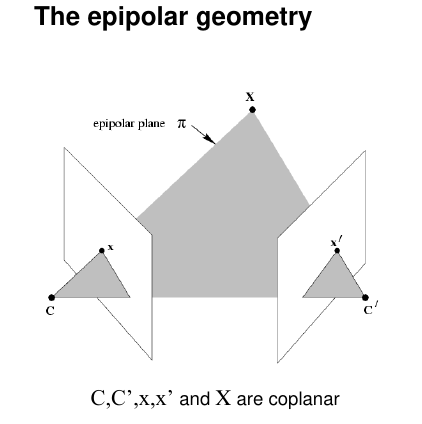
\includegraphics[width=0.8\linewidth]{epipolar_geometry}
\end{figure}

\subsection{The fundamental matrix F}

Samples can be arranged into A, which solves the equation \( A \boldsymbol{f} =
0\)
\[ 
    A = \begin{bmatrix}
        x_1' x_1 & x_1' y_1 & x_1' & y_1' x_1 & y_1' y_1 & y_1' & x_1 & y_1 & 1
        \\ \vdots \\
        x_n' x_n & x_n' y_n & x_n' & y_n' x_n & y_n' y_n & y_n' & x_n & y_n & 1
    \end{bmatrix}
\]
In the minimum, 7-point case, n is of course 7.

From A we can get F1 and F2 matrices, which come from the last two columns of
the V (SVD) of A.

From F1 and F2 we calculate the eigenvalues \( \lambda =
\operatorname{eig}(F_2^{-1} F_1) \). Only the real values are possible
solutions. Finally, we can get the fundamental matrix from \( F = F_1 \lambda
F_2 \)

\subsection{The essential matrix}

E can be derived from F by \( E = K'^T F K \)

\subsection{Triangulation}

Points should be normalized and denormalized as with the H computation.
First, form \(P\) and \(P'\).
\[
    P = K[I | 0]
\]
\[
    P' = K'[R | T]
\]

Once again, form A 
\[
    A = \begin{bmatrix}
        x \boldsymbol{p}^{3T} - \boldsymbol{p}^{1T} \\
        y \boldsymbol{p}^{3T} - \boldsymbol{p}^{2T} \\

        x' \boldsymbol{p}'^{3T} - \boldsymbol{p}'^{1T} \\
        y' \boldsymbol{p}'^{3T} - \boldsymbol{p}'^{2T} \\
    \end{bmatrix}
\]
Where \( \boldsymbol{p}^{iT} \) are rows of \(P\).

The points can be retrieved from the last column of V, of the SVD of A.
































